
\chapter{Spannkraftinduzierten Deformation}

Im folgenden Kapitel wird die Methode zur Erkennung und Analyse von durch 
Spannkraft induzierten Deformationen erläutert. Ziel ist es, 
Deformationen anhand von zwei zusammengefügten Bildern aus unterschiedlichen 
Spannungsstufen zu identifizieren. Eine Deformation wird als äußerliche 
Veränderung des betrachteten Bauteils definiert, wobei diese Veränderung 
durch den Unterschied der Ränder der Bauteile bestimmt wird.
Bevor eine Deformation erkannt werden kann, muss die Randgeometrie beider 
abgebildeter Bauteile erfasst werden. 
Zunächst werden in einem Schritt immer zwei Spannungsstufen miteinander verglichen,
und die Deformationsdaten anschließend gespeichert. 
Die Auswertung der resultierenden Daten erfolgt in einem separaten Schritt, 
wodurch es möglich ist, mehrere Spannungsstufen miteinander zu vergleichen,
ohne dass die Komplexität des Verfahrens ansteigt.

\section{Deformation zwischen zwei Spannungszuständen}

Wie beschrieben, wird die Deformation zwischen zwei Bauteilen als Differenz 
der Randgeometrie definiert. Um die Randgeometrie eines Bauteils zu ermitteln, 
kann erneut die Kontursuche (In Kapitel~\ref{contoursearching} beschrieben)
angewendet werden. 
Die ermittelten Konturen bilden die Ränder des Bauteils ab und 
erfassen sowohl äußere als auch innere Geometrien, was 
die Deformationserkennung ermöglicht. In Abbildung~\ref{fig:stichted_contour} 
ist ein zusammengefügtes Bild sowie die erkannte Randgeometrie eines 
Bauteils dargestellt.

\begin{figure}[H]
    \centering
    \begin{minipage}{0.49\textwidth}
        \centering
        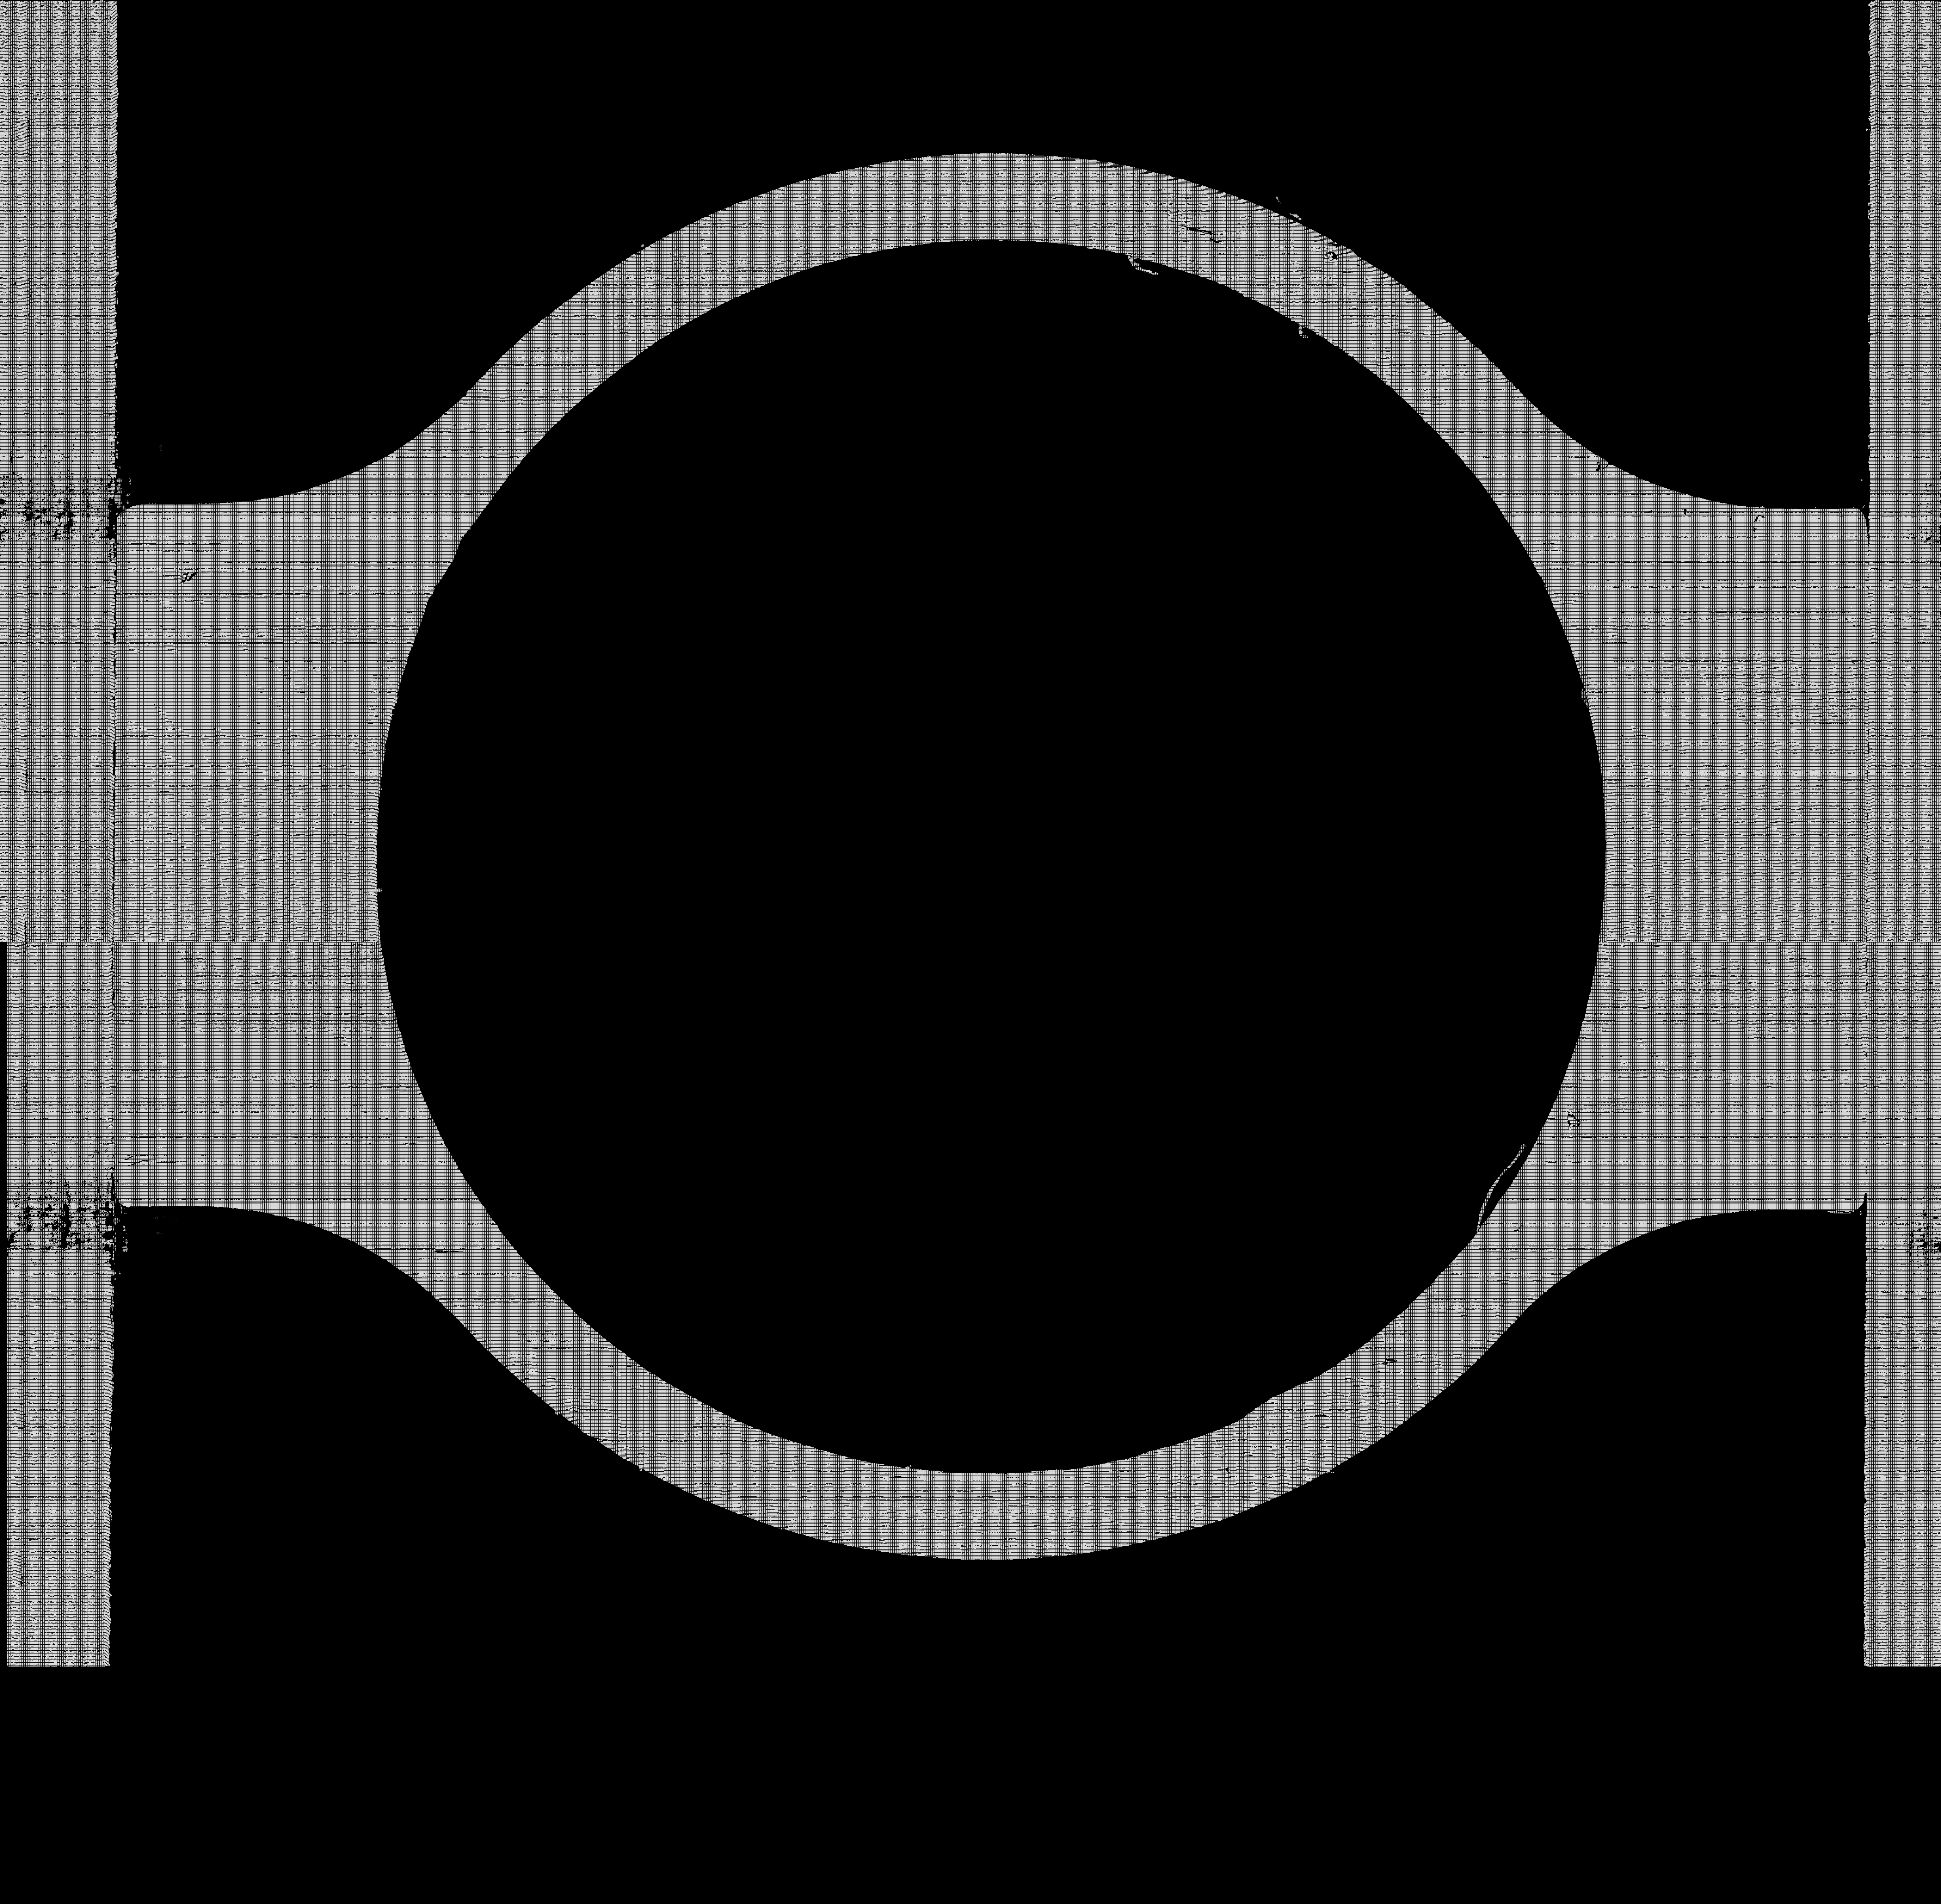
\includegraphics[width=\textwidth]{images/FDM2_SP0_stitched.png} % first figure itself
        \caption*{(a)} 
    \end{minipage}\hfill
    \begin{minipage}{0.49\textwidth}
        \centering
        \includegraphics[width=\textwidth]{images/contours_FDM2_SP0_stitched.png} % first figure itself
        \caption*{(b)}
    \end{minipage}\hfill
    \caption{(a) Zusammengefügtes Bild des FDM Demonstratorbauteils, Spannungsstufe 0
    (b) Randgeometrie von (a), die zur Erkennung der Deformation genutzt wird}
        \label{fig:stichted_contour}
\end{figure}

\section{Randgeometrien übereinander legen}

Um die Differenz zweier Randgeometrien bestimmen zu können, 
müssen diese präzise übereinander gelegt werden. Dies gewährleistet, 
dass die resultierende Differenz minimal ist. Der bereits beschriebene Ansatz 
des Konturmatchings (siehe Kapitel~\ref{contoursearching}) könnte auch hier genutzt werden. Allerdings 
müssen in diesem Fall die gesamten Konturen berücksichtigt werden und nicht 
nur der überlappende Ausschnitt. Das zuvor vorgestellte Verfahren ist jedoch 
für die Konturen eines gesamten Bauteils nicht performant genug, um eine 
akzeptable Laufzeit sicherzustellen.

Deshalb wird in diesem Kontext ein alternatives Verfahren eingesetzt. 
Es basiert auf dem Prinzip, Punktepaare zu finden, deren euklidische
Distanz gleich null ist. Anstatt jedoch jeden Punkt der Zielkontur mit 
jedem Punkt der Ursprungskontur zu vergleichen, wird ein maximaler Radius definiert, 
innerhalb dessen nach benachbarten Punkten gesucht wird. Hierfür muss die Kontur 
zunächst in eine zweidimensionale Datenstruktur überführt werden. Dieser zusätzliche 
Aufwand führt zu einer erheblichen Verkürzung der Laufzeit.

Ähnlich dem bereits in Kapitel \ref{icp} beschriebenen ICP-Algorithmus wird eine Transformation 
berechnet, die eine Kontur an eine andere annähert. Die Berechnung der 
Transformation erfolgt nach folgendem Algorithmus:

\begin{enumerate}
    \item Zu jedem Punkt in der Ursprungskontur wird der Nachbarpunkt
    in der Zielkontur gesucht, der den kleinsten euklidischen Abstand besitzt.
    \item Wird kein solcher Punkt in einem definierten Radius gefunden,
    wird der nächste Punkt der Ursprungskontur
    betrachtet. Falls ein Punkt gefunden wurde, wird der Vektor gebildet der die Punkte
    der Ursprungs- und Zielkontur verbindet.
    \item Wenn alle Punkte der Ursprungskontur betrachtet sind, wird der 
    Durchschnitt aller gefunden Vektoren gebildet.
    \item Da die Transformation auf Pixel angewendet wird, muss sie ganzen Zahlen 
    entsprechen. Wenn der Absolutwert beider Vektorelemente der Transformation 
    unter 0.2 Pixel fällt wird die Transformation auf (0, 0) gerundet.
    Ansonsten wird auf die nächste ganze Zahl gerundet.
\end{enumerate}

Ist die Transformation ungleich dem Vektor (0, 0) wird sie auf die Ursprungskontur 
angewendet und erneut die Transformation berechnet. Dies wird so lange wiederholt bis 
die Transformation dem Nullvektor entspricht. Wenn dies geschieht, sind beide Konturen, 
und damit die Randgeometrien der Bauteile angenähert.
Um Rechenzeit zu sparen werden vor dem Ermitteln der ersten Transformation die 
Massenmittelpunkte beider Bauteilgeometrien berechnet und beide Bilder so transformiert, 
dass sie den gleichen Massenmittelpunkt haben.
In Abbildung~\ref{fig:stichted_contours_compare} sind die Konturen vor und nach 
dem Überlappungs-prozess abgebildet.

\begin{figure}[H]
    \centering
    \begin{minipage}{0.49\textwidth}
        \centering
        \includegraphics[width=\textwidth]{images/contours_before_matching2.png} % first figure itself
        \caption*{(a)} 
    \end{minipage}\hfill
    \begin{minipage}{0.49\textwidth}
        \centering
        \includegraphics[width=\textwidth]{images/contours_matching_13.png} % first figure itself
        \caption*{(b)}
    \end{minipage}\hfill
    \caption{(a) Die Konturen von zwei Bauteilen vor dem übereinanderlegen. 
    (b) Die Konturen, nachdem sie mit dem Vorgestellen Verfahren angenähert wurden.}
        \label{fig:stichted_contours_compare}
\end{figure}

\section{Deformation messen} \label{defoinfo}

Nachdem die beschriebenen Schritte erfolgt sind, kann die Deformation bestimmt werden.
Mit Deformation ist eine Änderung in der Randgeometrie des Bauteils gemeint.
Eine Deformierung kann an jedem Rand eines Bauteils auftreten.
Um die Deformation eines Bauteils zu messen, wird über die 
gesamte x-Achse des Bildes iteriert und die kleinste Differenz 
zwischen zwei Punkten gebildet. Diese entspricht dann einer Abweichung. 
Da innere und äußere Randgeometrie separat betrachtet werden, kann es immer nur zwei
solcher Punktepaare geben, eins am oberen Ende des Bauteils und eins am unteren Ende.
Es wird der euklidische Abstand beider Punktepaare gebildet und aufsummiert.
So entsteht ein Datensatz für ein Bild, 
dass die Differenz zweier Spannungsstufen ausgibt. In Abbildung~\ref{fig:deformation_data}
ist ein solcher Datensatz zu sehen. 

Innere und äußere Randgeometrien werden separat betrachtet und analysiert.
In Abbildung~\ref{fig:deformation_data_vis} ist die Deformation des inneren Kreises
visuell dargestellt. In Abbildung \ref{fig:deformation_data_graph} sind die 
Deformationswerte grafisch dargestellt. Ein negativer Deformationswert bedeutet eine 
Verschiebung nach außen. Ein positiver Wert bedeutet das sich das Bauteil nach 
innen verformt hat. Das Vorzeichen hängt davon ab, welche Spannungsstufe zuerst ausgewählt
wird. Wird die größere Spannungsstufe mit einer kleineren verglichen, sind die Ergebnisse
invertiert.

Es wurde ein per FDM gefertigtes Bauteil eingespannt und zwei Spannungsstufen verglichen.
Die blaue Linie bildet die Randgeometrie des Bauteils ab, dass mit Spannungsstufe
null eingespannt wurde. Das entspricht hier nur einer lockerer Einspannung in den 
Schraubstock. Die magenta gefärbte Linie ist die Spannungsstufe sechs des gleichen
Bauteils. Hier wurde der Schraubstock mit einer Kraft von ca. 250 nm angezogen.

\begin{figure}[H]
    \centering
    \includegraphics[width=0.99\textwidth]{images/FDM2_SP0_stitched_FDM2_SP4_stitched_1_1_cut.png}
    \caption{Deformation der inneren Bauteilgeometrie des Demonstratorbauteils 
    visuell dargestellt}
    \label{fig:deformation_data_vis}
\end{figure}

\begin{figure}[H]
    \centering
    \includegraphics[width=0.9\textwidth]{images/FDM_sp0_sp4_inner.png}
    \caption{Deformation der inneren Bauteilgeometrie 
    des Demonstratorbauteils als Graph}
    \label{fig:deformation_data_graph}
\end{figure}

Es ist gut zu erkennen, dass sich das Bauteil 
im mittleren Bereich ausgedehnt hat und in den Randbereichen schmaler geworden ist.
Dieser Datensatz unterliegt einer relativ großen Streuung. Um mehrere Spannungsstufen
zu vergleichen, wird der Datensatz zu einer Geraden zusammengefasst.
Diese Gerade ist auch in Abbildung~\ref{fig:deformation_data} in blau zu sehen. Sie wird 
gebildet, indem immer zehn Datenpunkte zu einem zusammengefasst werden. 
So können auch mehrere Spannungsstufen visuell dargestellt und verglichen werden.

\begin{figure}[H]
    \centering
    \includegraphics[width=0.7\textwidth]{images/FDM_sp0_sp3_defo_plot.png}
    \caption{Differenz von zwei Spannungsstufen bei einem FDM Bauteil, äußere 
    Bauteilgeometrie.}
    \label{fig:deformation_data}
\end{figure}

\begin{figure}[H]
    \centering
    \includegraphics[width=0.7\textwidth]{images/FDM_sp0_many_defo_plot2.png}
    \caption{Differenz von mehreren Spannungsstufen bei einem FDM Bauteil}
    \label{fig:deformation_data_all}
\end{figure}



